\section{Electronics}\label{sec:electronics}
% Small introduction to tikz figures and its basics, can be found on 
% http://cremeronline.com/LaTeX/minimaltikz.pdf
% Under the file tikz_magic.tex all the different boxes can be found!
%\subsection{Single board reconfigurable I/O}

The electronic setup \cite{Chris_Surgical} contains a \textbf{Single Board Reconfigurable Input/Output 9636} (sbRIO) controller, see \figref{fig:sbRIO9636}, which is responsible for interfacing between the surgical robot and the computer running ROS, see \secref{sec:ros}. It reads the sensor measurements, sends them to the PC and controls the motors based on the received reference signals. The sbRIO has built in safety protocols that disable the motors in case of error.

\begin{figure}[H]
	\centering
		\centering
		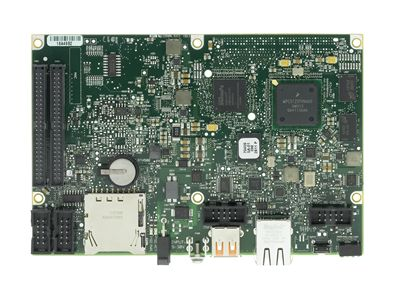
\includegraphics[width=0.7\linewidth]{sbRIO9636.jpg}
		\caption{The sbRIO 9636 board\cite{sbRIO9636Pic}}
		\label{fig:sbRIO9636}
\end{figure}


The controller consists of
\begin{itemize}
	\item 400 MHz real time processor
	\item 256 MB of system memory and 512 MB nonvolatile memory
	\item Reconfigurable Xilinx Spartan-6 LX45 FPGA
	\item 16 bit analog and digital I/O
	\item Built in USB, CAN, 10/100 Mb/s Ethernet peripherials
\end{itemize}

The board is configured through ethernet cable. The programs can be written in Labview, C or C++. We used LabView code to operate the sbRIO. The board is capable of running Real-time. %code, which is unmatched on the ROS side.

% http://sine.ni.com/nips/cds/view/p/lang/en/nid/210421

\subsection{Hardware setup}

The Endowrists, see \figref{fig:endowrits_set}, is actuated by 4 Maxon DC motors, see \secref{Maxon_Motor}. Each motor is equipped with an ESCON motor controller responsible for the cascade speed and inner loop current control. The control reference is sent through the sbRIO. They also provide current measurements to the sbRIO. Each motor hosts an encoder and a potmeter that provide absolute and relative angular position information to the FPGA built into the sbRIO board. For a graphical illustration of the connection see \figref{electro_setup}.
 
\todo{som explanation for the next line UDP, or erase it?}
The sbRIO communicates with the PC using UDP protocol. 

%\begin{figure}[H]
\begin{tikzpicture}

\node[state] (Endowrist) 
{
	%\parbox[c][2cm][c]{4cm}{\hspace{2.5em} \textbf{Endowrist}}
	\parbox[c][1.5cm][c]{2cm}{\textbf{Endowrist}}
};

\node[state,       % layout (defined above)
node distance=4cm,     
right of=Endowrist,        % Position is to the right of QUERY
yshift=+1cm] (Sensors)    % move 3cm in y
{%                     % posistion relative to the center of the 'box'
	\parbox[c][1.5cm][c]{2cm}{\textbf{Potmeters \\Encoders}}
};

\node[state,       % layout (defined above)
node distance=4cm,     
text width=4cm,        % max text width
right of=Endowrist,        % Position is to the right of QUERY
yshift=-1.5cm] (Escon)    % move 3cm in y
{%                     % posistion relative to the center of the 'box'
	\textbf{Escon controller}\\
	
	Speed control\\
	Current control\\
	Current measurement
};

\node[state,       % layout (defined above)
node distance=9.5cm,     
text width=5cm,        % max text width
right of=Endowrist,        % Position is to the right of QUERY
yshift=-0.5cm] (sbRIO)    % move 3cm in y
{%                     % posistion relative to the center of the 'box'
	\textbf{sbRIO}\\	
	 
	 .\newline\newline\newline
	
	Get control reference
	Get measurement data
	Communicate with PC\\
	
	
	
};

\node[state,       % layout (defined above)
node distance=9.5cm,     
text width=4cm,        % max text width
right of=Endowrist
] (FPGA)    % move 3cm in y
{%                     % posistion relative to the center of the 'box'
	\textbf{FPGA}\\
	
	Interface with the encoders and potmeters
	};

% draw the paths and and print some Text below/above the graph
\path (Endowrist) 	edge[bend left=20]  node[anchor=south,above]{}
node[anchor=north,below]{} (Sensors)
(Endowrist)     	edge[bend right=20] node[anchor=south,above]{} (Escon)
(Escon) edge[bend right=10] node[anchor=south,above]{} (sbRIO)
(Sensors) edge[bend left=10] node[anchor=south,above]{} (FPGA)
;


\end{tikzpicture}
\caption{Overwiev of the electronic components}
\label{electro_setup}
\end{figure} % Old picture
% \begin{figure}[H]
% \centering
% \begin{tikzpicture}
% %\draw (-1.5,-1.5) rectangle (13.5,1.5);

% \draw (-2.8,3.1) rectangle (2.8,-12.8);
% \node at (0,2.5) {\textbf{sbRIO}};


% \draw (-2.5,2) rectangle (2.5,-4.2);
% \node at (0,1.5) {\textbf{Micro processor}};
% \node[box] (datlog) at (0,0.3) {Data logging};
% \node[box] (ethcommu) at ($(0,-1.7) + (datlog)$) {Ethernet communication};
% \node[box] (shuterr) at ($(0,-1.7) + (ethcommu)$) {Shutdown:\\Communication error};


% \draw (-2.5,-4.7) rectangle (2.5,-12.6);
% \node at (0,-5.2) {\textbf{FPGA}};
% \node[box] (poscon) at ($(0,-3.3) + (shuterr)$) {Position control};
% \node[box] (enco) at ($(0,-1.7) + (poscon)$) {Encoder counter};
% \node[box] (PWM) at ($(0,-1.7) + (enco)$) {PWM control};
% \node[box] (dataES) at ($(0,-1.7) + (PWM)$) {Read data: ESCON};


% \draw (-9,-6) rectangle (-4,-12.6);
% \node[box] (spcon) at (-6.5,-8) {Speed control\\with inner current\\control};
% \node at ($(spcon) + (0,1.5)$) {\textbf{ESCON}};
% \node at ($(spcon) + (0,1.2)$) {\textbf{motor controller}};
% \node[box] (limcu) at ($(0,-1.7) + (spcon)$) {Limit output\\current};
% \node[box] (reen) at ($(0,-1.7) + (limcu)$) {Read encoder\\ticks};


% \draw (-9,-5.5) rectangle (-4,-4);
% \node at (-6.5,-4.75) {\textbf{Motor}};


% \draw (-9,-3.5) rectangle (-4,3.1);
% \node at (-6.5,2.5) {\textbf{ROS computer}};

%\node[fill = {rgb:red,1;green,2;blue,5},box] (Opt) at (0,0) {Operator};
%\node[fill = {rgb:red,1;green,2;blue,5},box] (Geo) at ($(3,0) + (Opt)$) {};
%\node[fill = {rgb:red,1;green,2;blue,5},box] (ros) at ($(3,0) + (Geo)$) {Robotic\\operating\\system};
%\node[fill = {rgb:red,1;green,2;blue,5},box] (davin) at ($(3,0) + (ros)$) {Da Vinci\\robot};
%\node[fill = {rgb:red,1;green,2;blue,5},box] (end) at ($(3,0) + (davin)$) {Endowrist};


%\draw[->, ultra thick] ([yshift=0.3cm]Opt.east) -- ([yshift=0.3cm]Geo.west);
%\draw[->, ultra thick] ([yshift=0.3cm]Geo.east) -- ([yshift=0.3cm]ros.west);
%\draw[->, ultra thick] ([yshift=0.3cm]ros.east) -- ([yshift=0.3cm]davin.west);
%\draw[->, ultra thick] ([yshift=0.3cm]davin.east) -- ([yshift=0.3cm]end.west);


%\draw[<-, ultra thick] ([yshift=-0.3cm]Opt.east) -- ([yshift=-0.3cm]Geo.west);
%\draw[<-, ultra thick] ([yshift=-0.3cm]Geo.east) -- ([yshift=-0.3cm]ros.west);
%\draw[<-, ultra thick] ([yshift=-0.3cm]ros.east) -- ([yshift=-0.3cm]davin.west);
%\draw[<-, ultra thick] ([yshift=-0.3cm]davin.east) -- ([yshift=-0.3cm]end.west);

%\node at (1.5,1) {Position};
% \node at (4.5,1) {Position};
% \node at (7.5,1) {yes};
% \node at (10.5,1) {yes};

%\node at (1.5,-1) {Force};
% \node at (4.5,1) {Position};
% \node at (7.5,1) {yes};
% \node at (10.5,1) {yes};
%\end{tikzpicture}
%\caption{Overall system with feedback in both direction}
%\end{figure}



\begin{figure}[H]
\centering
\tikzset{dataset/.style = {rectangle, draw, text width = 5.5cm, minimum height=3cm}}
\begin{tikzpicture}

\node [dataset] (mpro) at (0,3) {\textbf{Micro processor}
\begin{itemize}[itemsep=0pt,partopsep=0pt,topsep=0pt]
\item Data logging
\item Ethernet communication
\item Shutdown: Communication error \\
\end{itemize}};

\node [dataset, below of=mpro, node distance=6.5cm] (FPGA) {\textbf{FPGA}
\begin{itemize}[itemsep=0pt,partopsep=0pt,topsep=0pt] 
\item Position contron
\item Encoder counter
\item PWM control
\item Read data: Escon 
\end{itemize}};

\draw[->, ultra thick] ([xshift=-1cm]mpro.south) -- ([xshift=-1cm]FPGA.north);
\draw[<-, ultra thick] ([xshift=1cm]mpro.south) -- ([xshift=1cm]FPGA.north);

\node [dataset, left of=FPGA, node distance=7cm] (emc) {\textbf{ESCON motor controller}
\begin{itemize}[itemsep=0pt,partopsep=0pt,topsep=0pt] 
\item Speed controll with intter current control
\item Limit output current
\item Read encoder ticks 
\end{itemize}};

\draw[->, ultra thick] ([yshift=-1cm]emc.east) -- ([yshift=-1cm]FPGA.west);
\draw[<-, ultra thick] ([yshift=1cm]emc.east) -- ([yshift=1cm]FPGA.west);

\tikzset{dataset/.style = {rectangle, draw, text width = 6cm, minimum height=10.5cm}}
\node [dataset, above of=FPGA, node distance=3.5cm] (motor) {\textbf{sbRIO}
\begin{itemize}[itemsep=0pt,partopsep=0pt,topsep=260pt] % Edit the last number to fit title 
\item[]  %  This line is necessary!!
\end{itemize}};


\tikzset{dataset/.style = {rectangle, draw, text width = 5.5cm, minimum height=1cm}}
\node [dataset, above of=emc, node distance=2.5cm] (motor) {\textbf{Motor}};

\draw[->, ultra thick] ([xshift=-1cm]motor.south) -- ([xshift=-1cm]emc.north);
\draw[<-, ultra thick] ([xshift=1cm]motor.south) -- ([xshift=1cm]emc.north);

\tikzset{dataset/.style = {rectangle, draw, text width = 5.5cm, minimum height=5cm}} % This edits the size of the Ros computer box 
\node [dataset, above of=motor, node distance=3.75cm] (ROS) {\textbf{Ros computer}
\begin{itemize}[itemsep=0pt,partopsep=0pt,topsep=0pt] 
\item 1
\item 2
\item 3 
\end{itemize}};

\draw[->, ultra thick] ([yshift=-1cm]mpro.west) -- ([yshift=-1cm]ROS.east); % ([yshift=-1cm]ROS.west) should probaly be edited!!!
\draw[<-, ultra thick] ([yshift=1cm]mpro.west) -- ([yshift=1cm]ROS.east);

% \draw [->,ultra thick] (-1,1.5) -- (-1,-2); %Micro to FPGA
% \draw [<-,ultra thick] (1,1.5) -- (1,-2);

% \draw [->,ultra thick] (-3,-3) -- (-4,-3);
% \draw [<-,ultra thick] (-3,-4) -- (-4,-4);

\end{tikzpicture}
\caption{Say somthing cool- "\textit{Somthing cool!}"}
\end{figure}

\todo{Include arrow, label anc new caption... elaborate this picture breifly, what do the different boxes do?}

% \begin{figure}[htb]
% \tikzset{dataset/.style = {rectangle, draw, text width = 5cm, minimum height=1in}}
% \begin{tikzpicture}[auto, font={\scriptsize}]
%     % Place nodes
%     \node [dataset] (tm) {Data 1 
%                             \begin{itemize}[itemsep=0pt,partopsep=0pt,topsep=0pt]   %% this added.
%                                 \item{\# Adults } 
%                                 \item{\# Children} 
%                                 \item{Income}
%                                 \item{Ethnicity}
%                             \end{itemize}\par};
%     \node [dataset, right of=tm, node distance=3in] (dmv) {Data 2 
%                             \begin{itemize}[itemsep=0pt,partopsep=0pt,topsep=0pt] 
%                                 \item{Data 2} 
%                             \end{itemize}\par};
%     % draw links
%     \path [<->] (tm) edge node[above, sloped] {Address} (dmv);
% \end{tikzpicture}
%     \caption{Analysis dataset assembly.}
%     \label{fig:dataset}
% \end{figure}


\subsection{Motor}\label{Maxon_Motor}
The four motors for actuating the Endowrist is sold as a bulk solution which include motor, gear and a position encoder, see \figref{fig:Full_motor _dis}.

The control of these motors are done through the ESCON motor drivers, which are connected to the sbRIO board. The datasheet for the motor parts can be found on \path{CD:/Datasheets/Motor/}\todo{(Datasheet) Don't know if this is necessary - Maby we don't have to turne in a physical paper??}

%The ESCON motor controllers are attached to the sbRIO controller and send the control signals through cables. The motor has a nominal torque of 6.96 mNm.
%4 Maxon motors are used for the actuation of the endowrist. The motors are implemented using a combination gear (Maxon 353816) including the gearing, the servo motor and the sensors. The ESCON motor controllers are attached to the sbRIO controller and send the control signals through cables. The motor has a nominal torque of 6.96 mNm.

\begin{figure}[H]
	\centering
	\begin{subfigure}{.32\textwidth}
		\vspace{0pt}
		\centering
		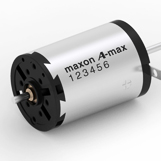
\includegraphics[width=\linewidth]{motor.jpg}
		\caption{The Maxon 110160 \newline DC motor\cite{motor_motor}}
		\label{fig:motor}
	\end{subfigure}
	\begin{subfigure}{.32\textwidth}
		\centering
		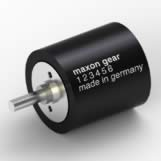
\includegraphics[width=\linewidth]{motor_gear.jpg}
		\caption{The planetary gearhead equipped with sleeve bearing\cite{motor_gear}}
		\label{fig:motor_gear}
	\end{subfigure}
	\begin{subfigure}{.32\textwidth}
	\hspace{5pt}
		\centering
		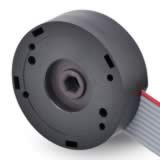
\includegraphics[width=\linewidth]{motor_sensor.jpg}
		\caption{The encoder used for getting angular data\cite{motor_encoder}}
		\label{fig:motor_sensor}
	\end{subfigure}
	\caption{The combination gear disassembled}
	\label{fig:Full_motor _dis}
\end{figure}





\subsection{ESCON 50/5 motor controller}
For driving the motors, there has been implemented four ESCON motor driver of the type 50/5 (part number 438725), see \figref{fig:ESCON505}. 

\begin{figure}[H]
	\centering
		\centering
		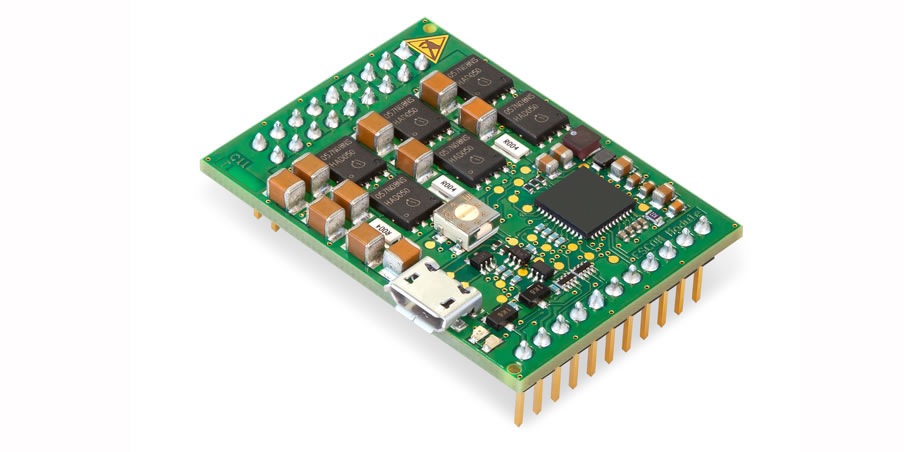
\includegraphics[width=0.7\linewidth]{ESCON505.jpg}
		\caption{ESCON 50/5 DC motor controller\cite{ESCON_motor_controller}}
		\label{fig:ESCON505}
\end{figure}

These are controllers for permanent magnet-activated bushed DC motors an can deliver a power up to 250 Watt for the motor connected to the controller. 

It has three operating modes

\begin{itemize}
\item Current controller
\item Speed controller (open loop)
\item Speed controller (closed loop)
\end{itemize}

The reason we chose speed controller with inner loop control is explained in \ref{Embedded}.



\section{Mechanical test setup}\label{sec:Mechanical_testsetup.tex}
The mechanical test setup available at Aalborg University can be seen on \figref{fig:Mec_abcd}. It includes four of the motors described in \secref{Maxon_Motor} attached to the four rotational plates seen on \figref{fig:Mec_a} and \figref{fig:Mec_b}. These plates connect the motors and the Endowrist, such that the EndoWrist can be manipulated. See \figref{fig:Mec_c} and \figref{fig:Mec_d} for the attachment of the Endowrist to the EndoWrist holder.  

\begin{figure}[H]
	\centering
	\begin{minipage}[t]{0.9\textwidth}
	\begin{subfigure}{0.45\textwidth}
		\vspace{-10pt}
		\centering
		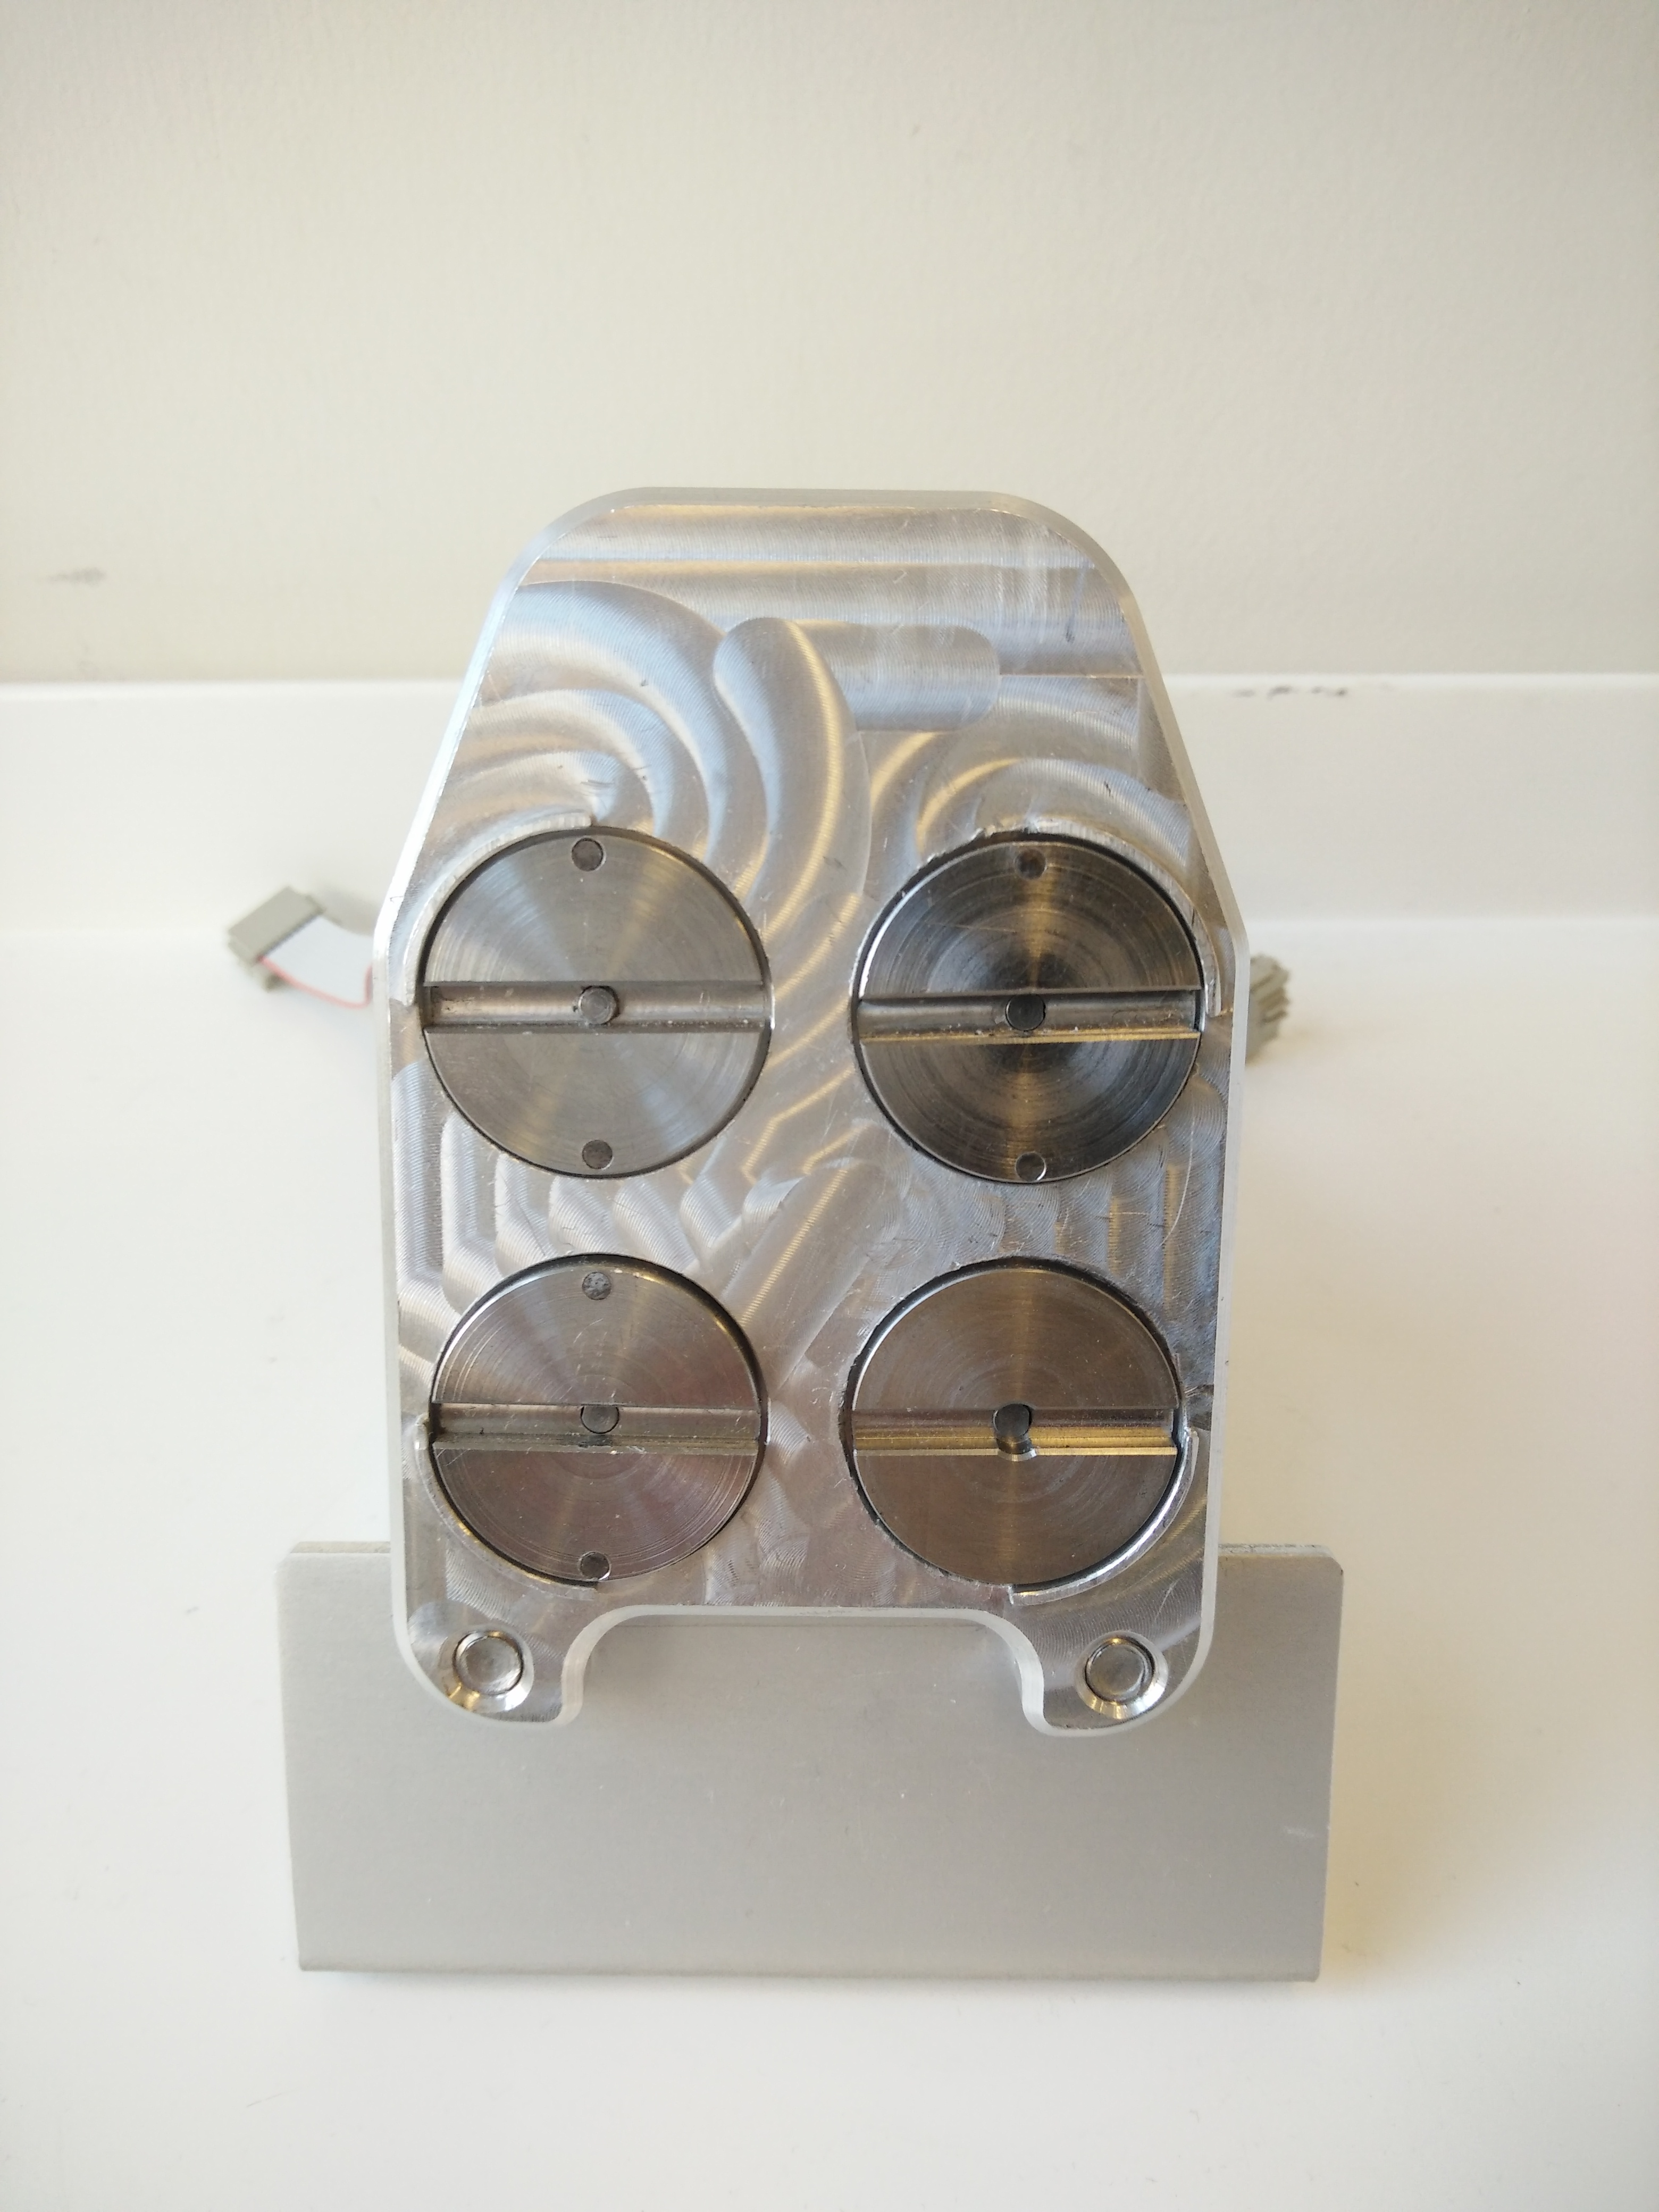
\includegraphics[width=\linewidth]{Test_setup1.jpg}
		\caption{EndoWrist holder. Front view}
		\label{fig:Mec_a}
	\end{subfigure}
	\hspace{\fill}
	\begin{subfigure}{0.45\textwidth}
		\centering
		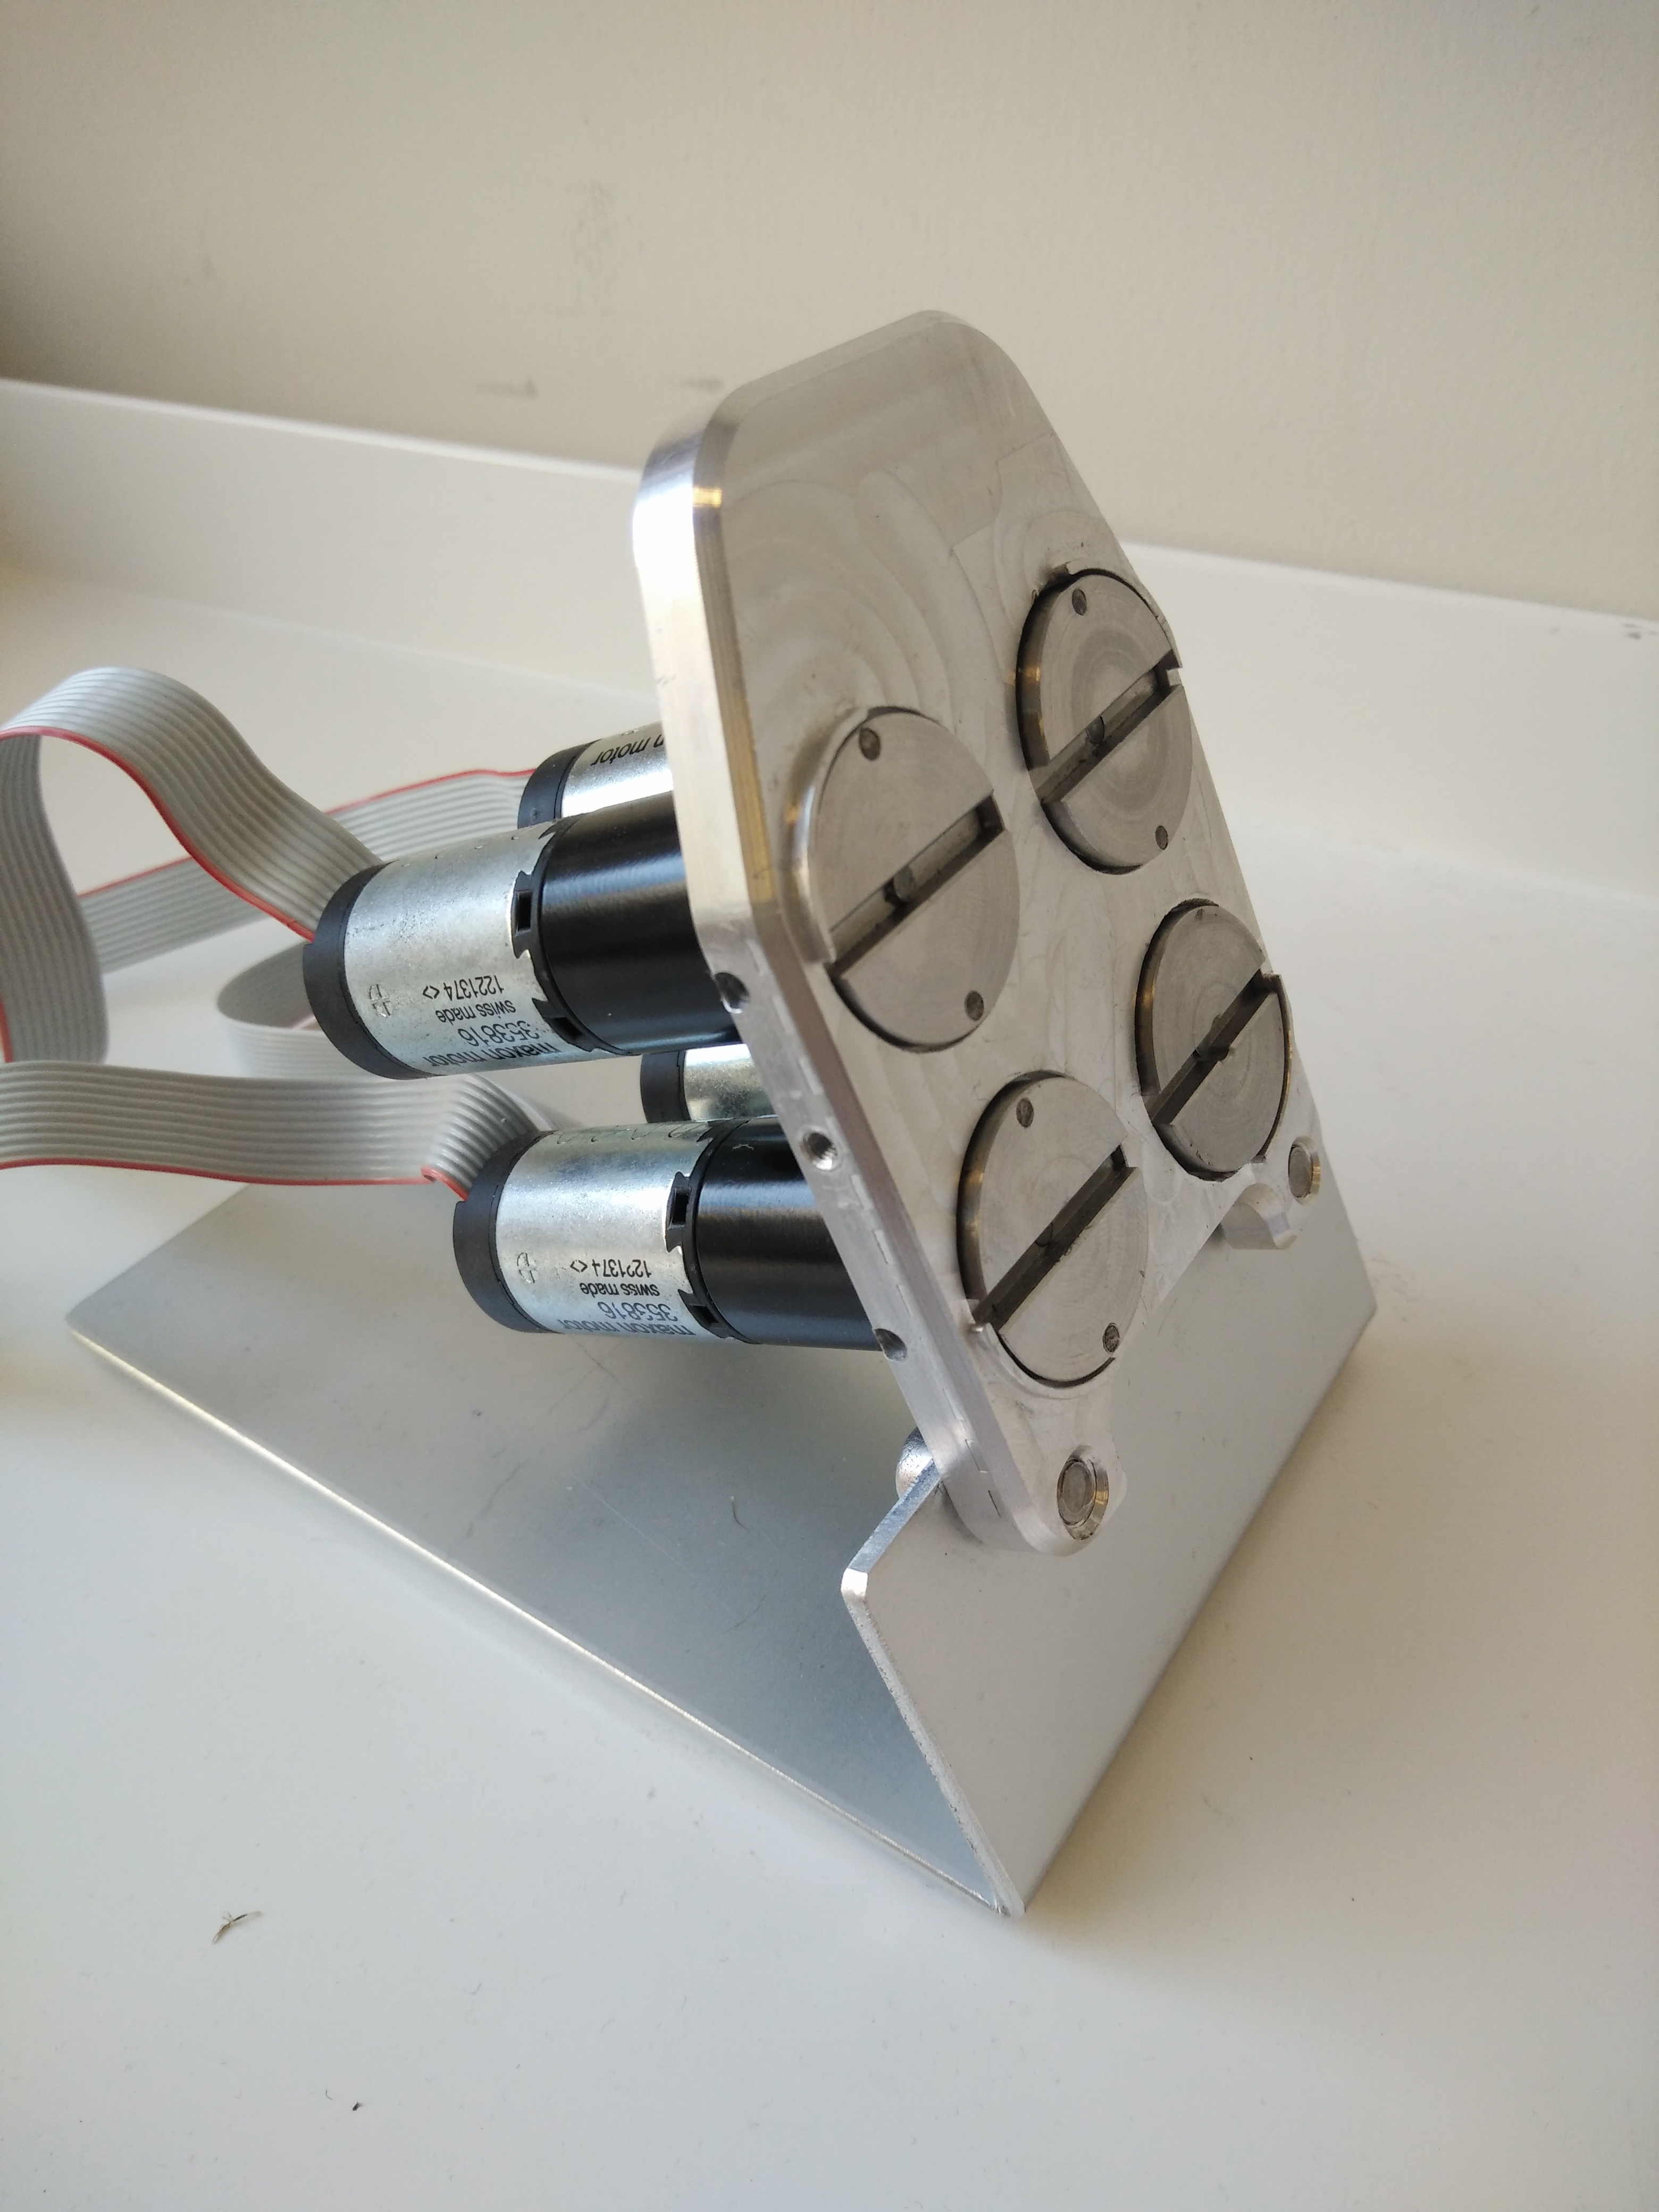
\includegraphics[width=\linewidth]{Test_setup2.jpg}
		\caption{EndoWrist holder with motors at the back. Side view}
		\label{fig:Mec_b}
	\end{subfigure}
	\end{minipage}

	\begin{minipage}[t]{0.9\textwidth}
	\vspace{20pt}
	\begin{subfigure}{0.45\textwidth}
		\vspace{0pt}
		\centering
		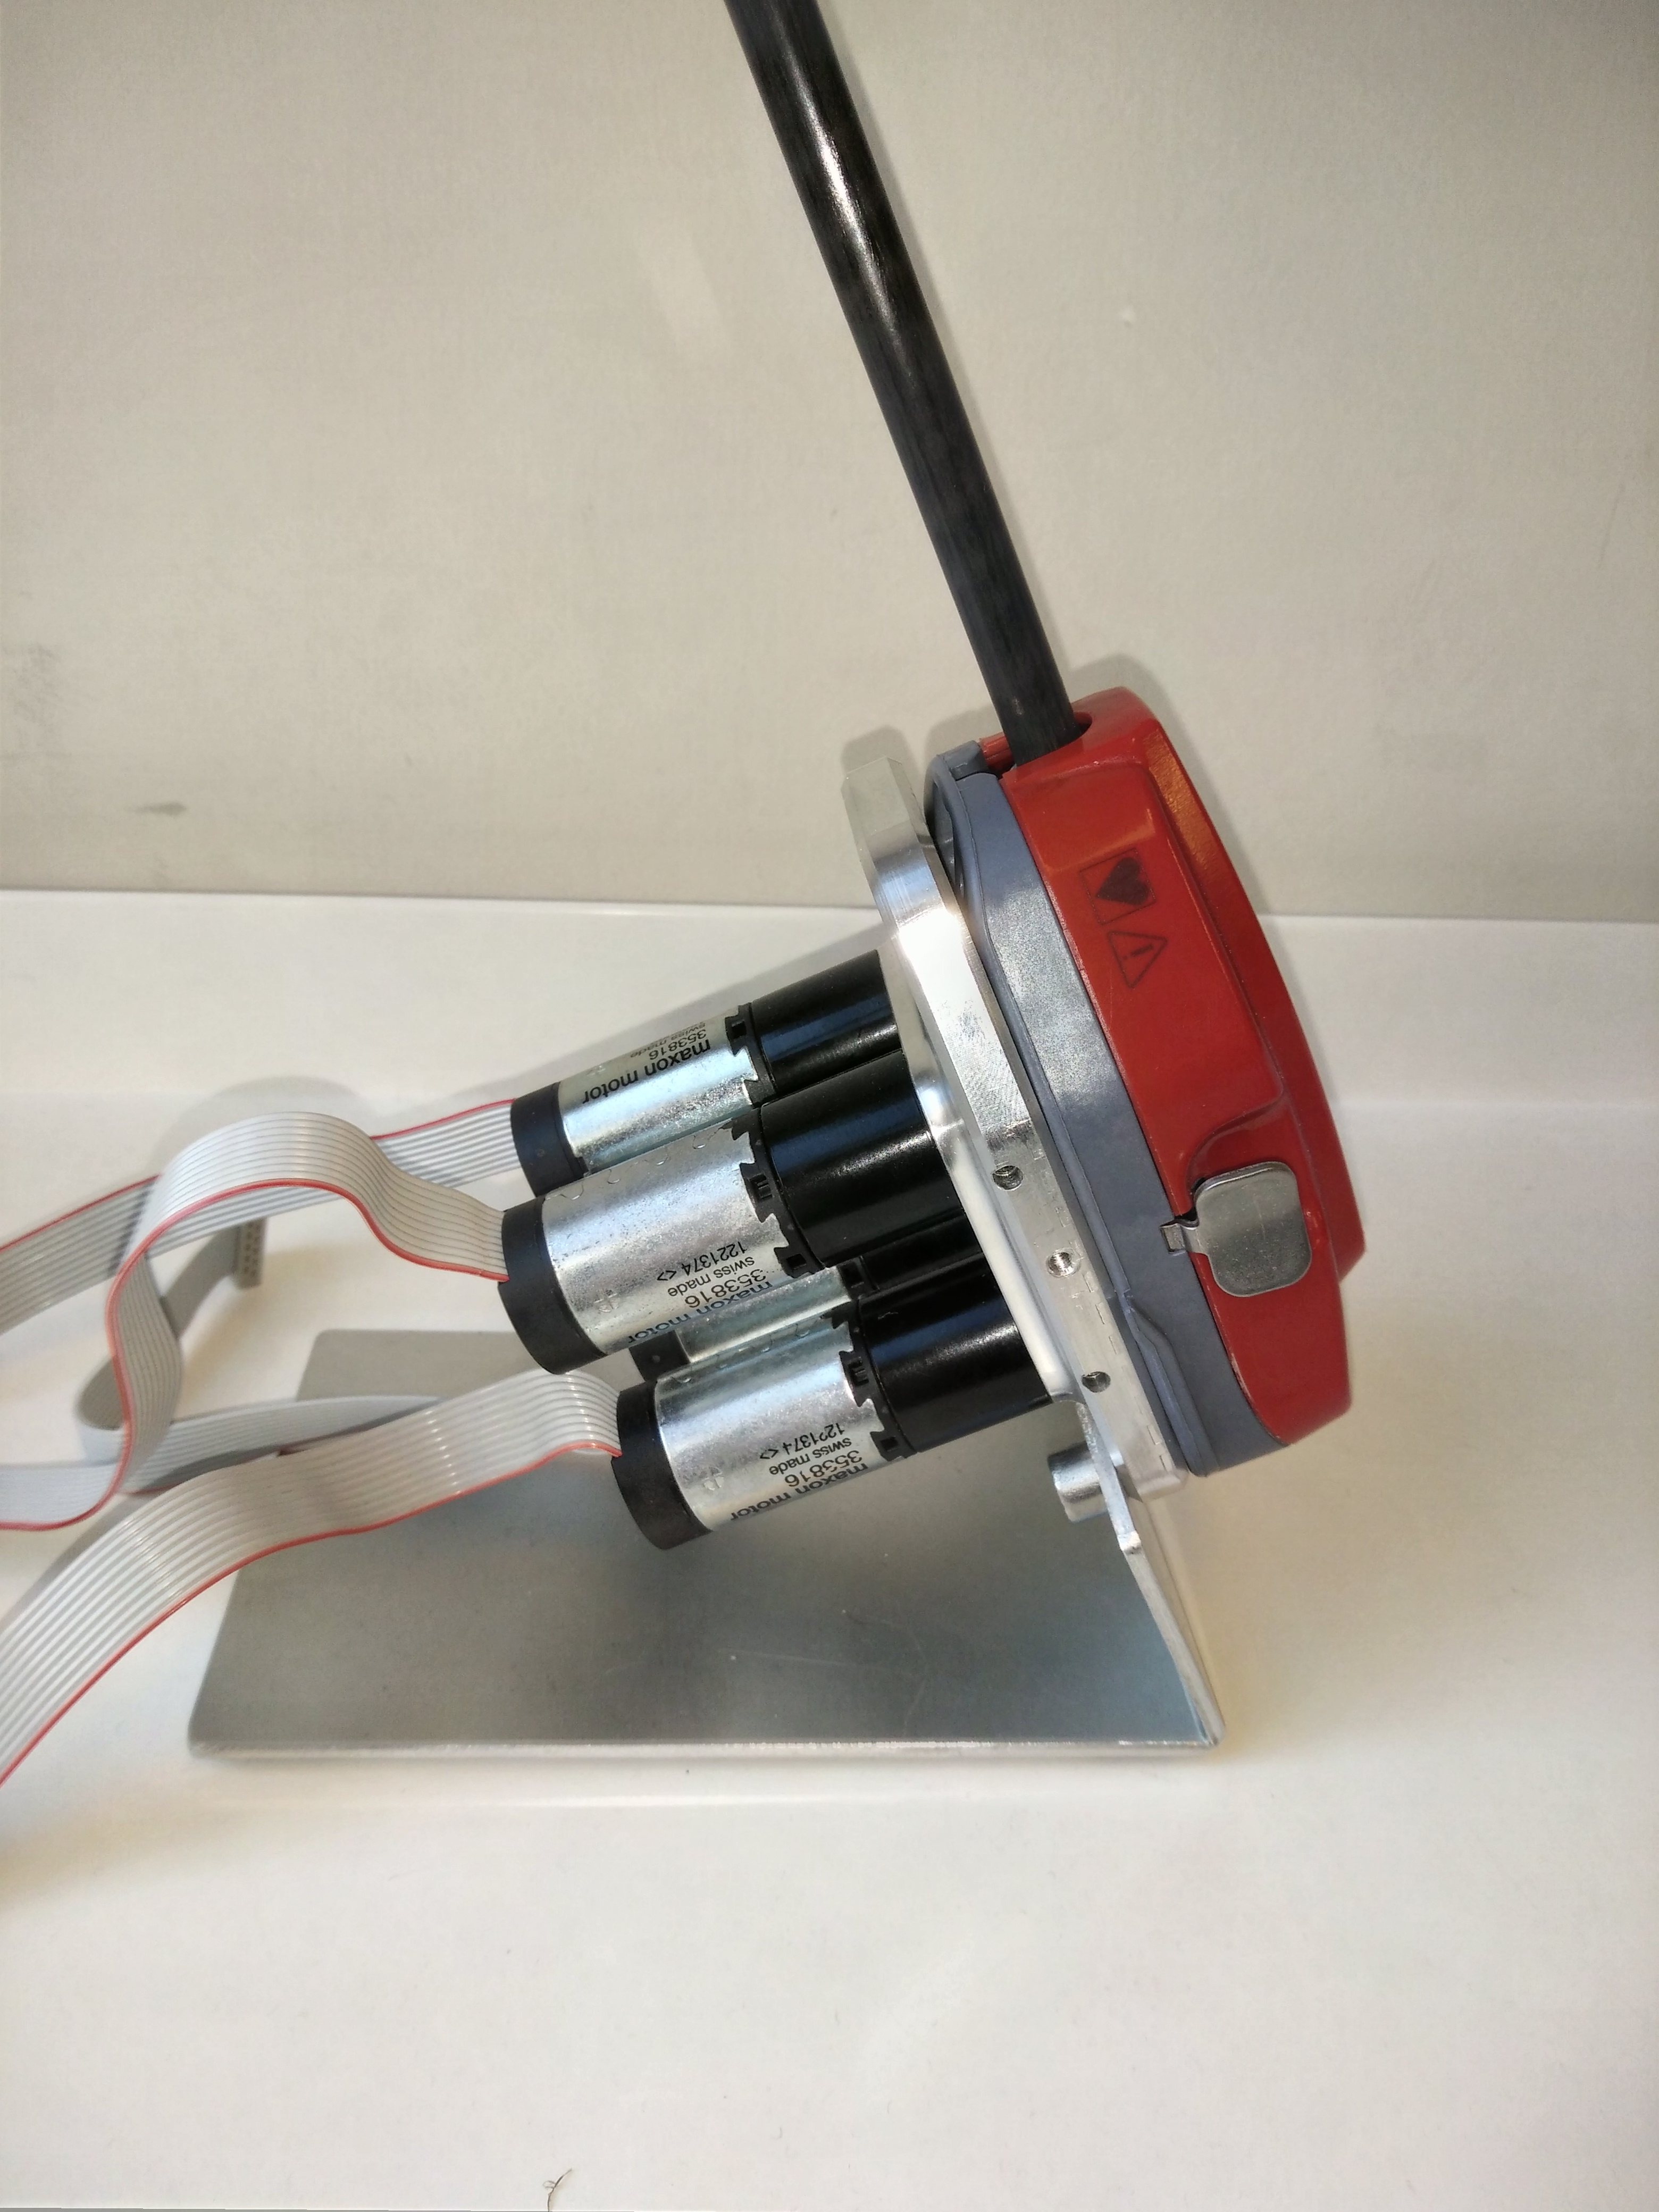
\includegraphics[width=\linewidth]{Test_setup3.jpg}
		\caption{EndoWrist holder with EndoWrist and motors. Side view}
		\label{fig:Mec_c}
	\end{subfigure}
	\hspace{\fill}
	\begin{subfigure}{0.45\textwidth}
		\centering
		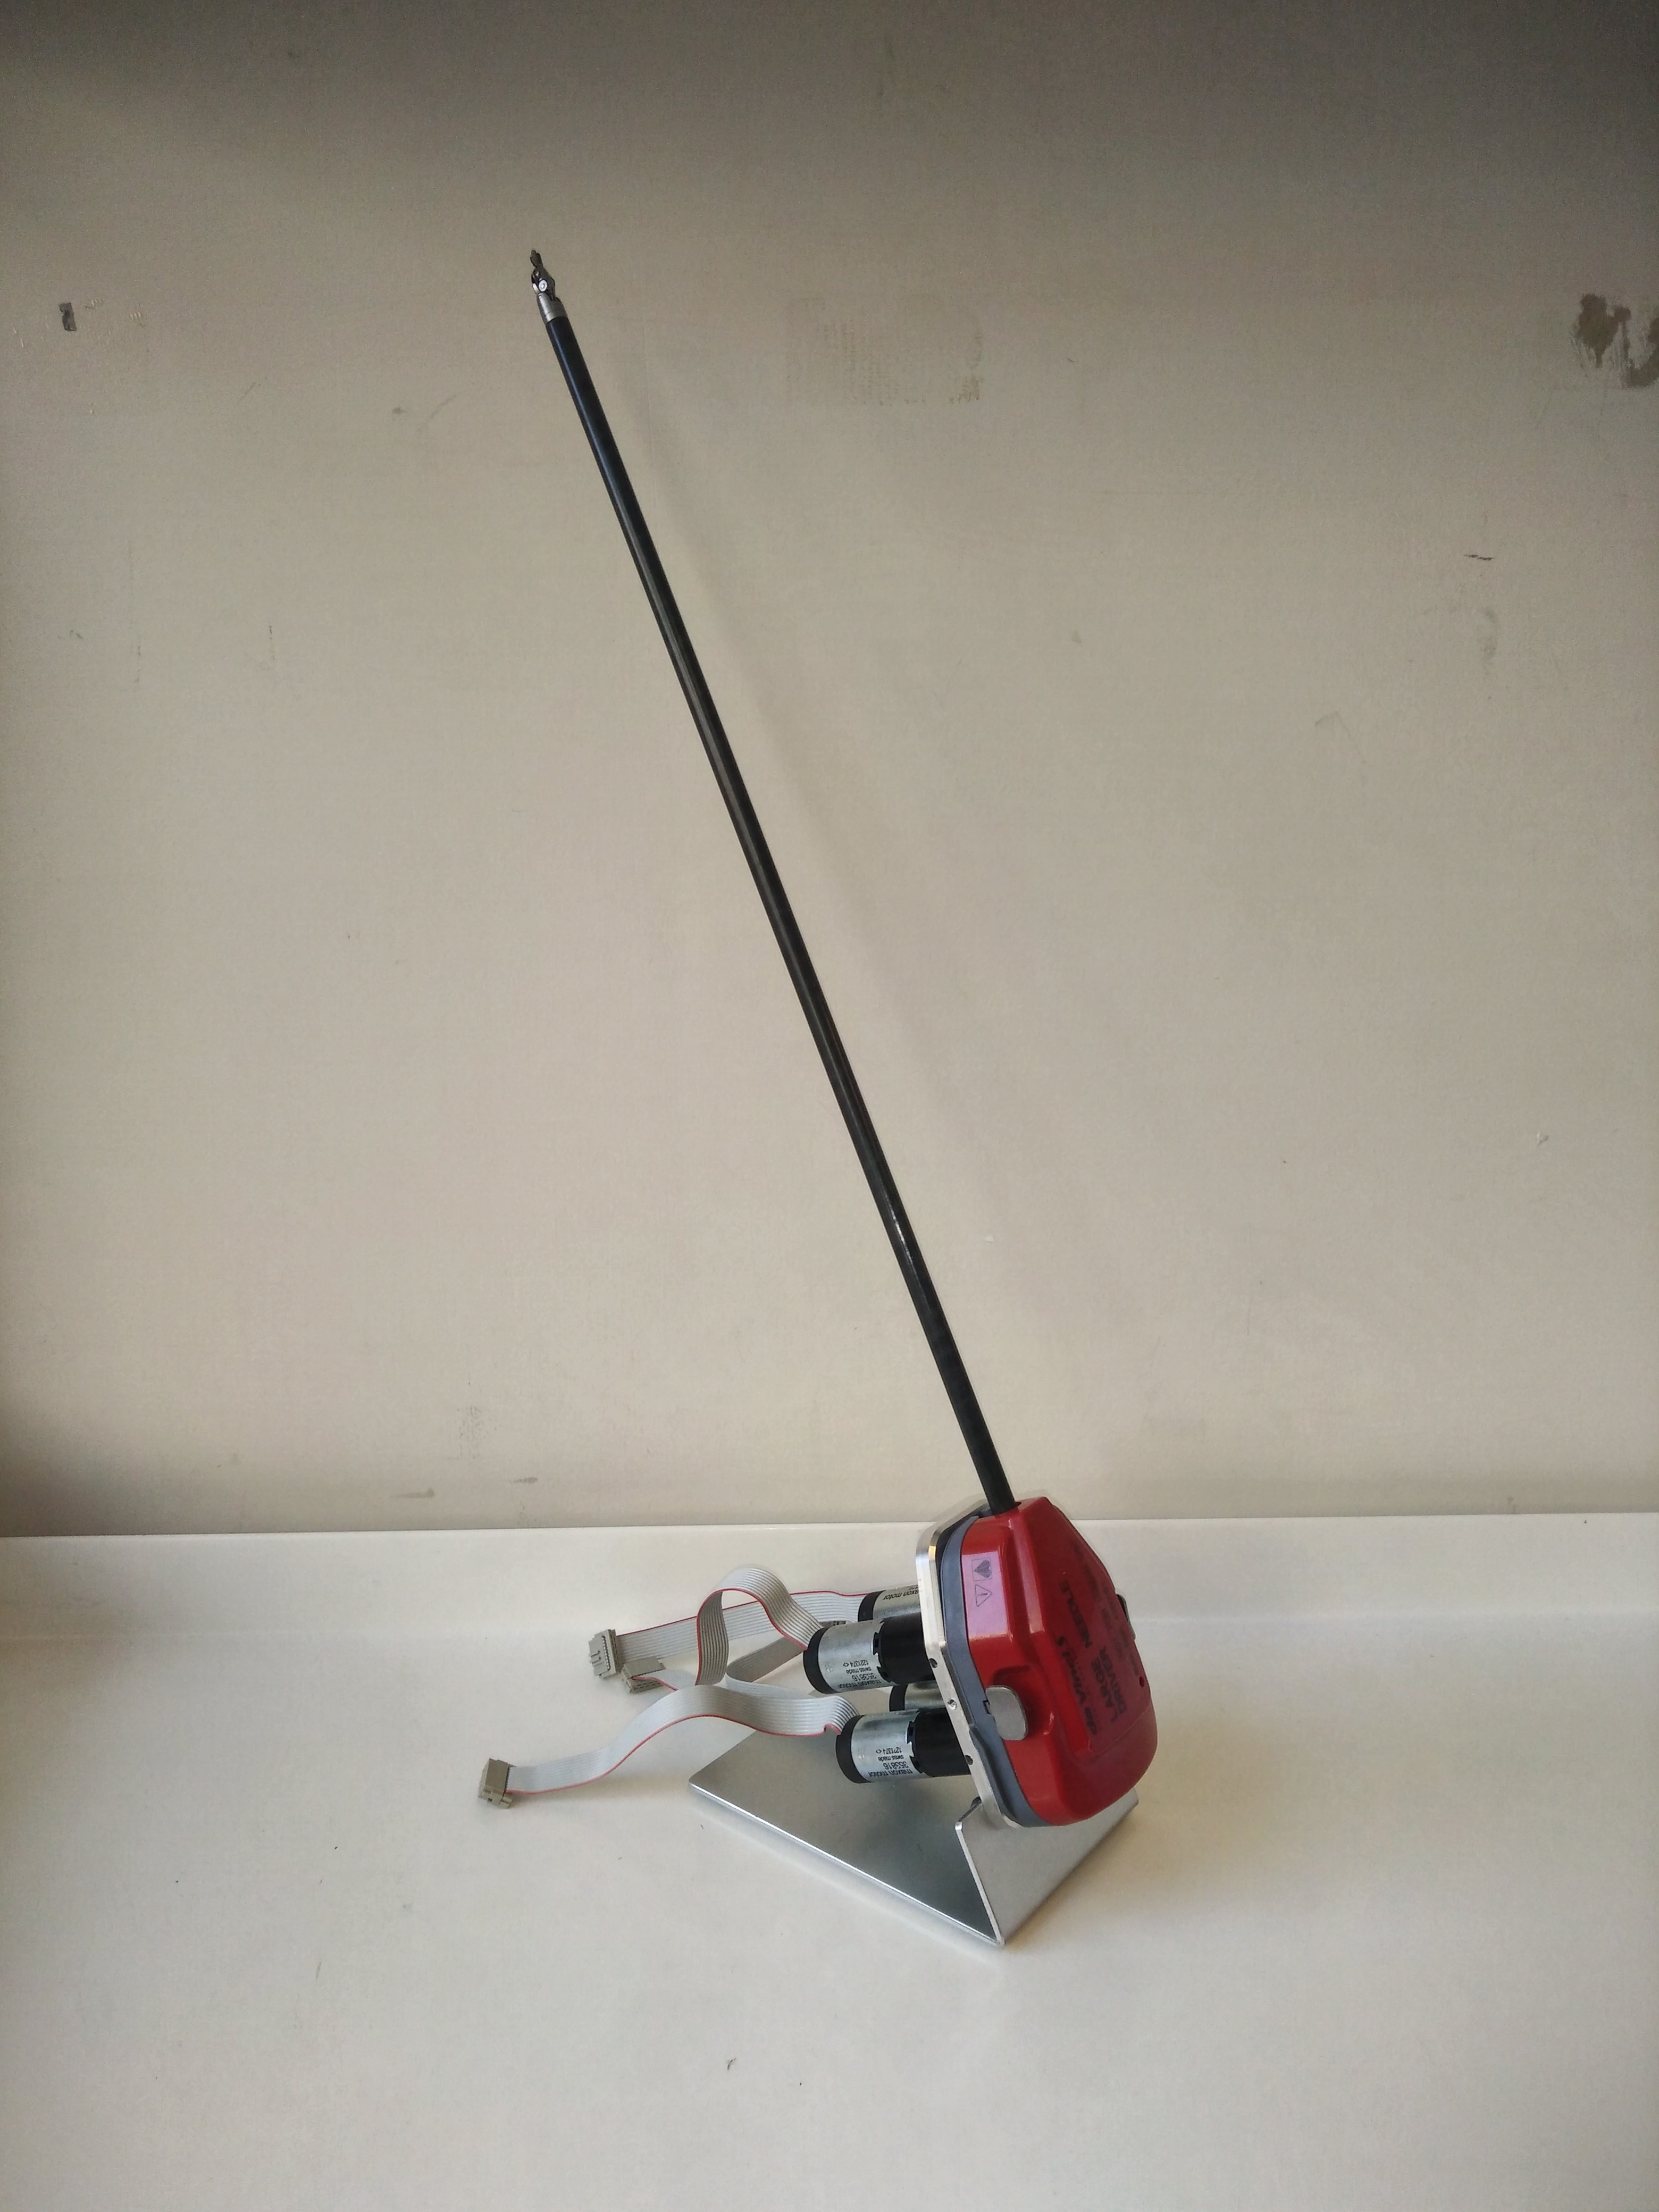
\includegraphics[width=\linewidth]{Test_setup4.jpg}
		\caption{Full view of the mechanical test setup}
		\label{fig:Mec_d}
	\end{subfigure}
	\end{minipage}

	\caption{Four pictures of the mechanical test setup available at Aalborg University, which include motors, EndoWrist and EndoWrist holder}
	\label{fig:Mec_abcd}
\end{figure}

This setup can manipulate the EndoWrist in the same manner as if the tool was connected to the da Vinci robot, see \secref{sec:da_vin_rob}.
\todo{Does this last line explaine what the setup can do in a proper manner?}
